\documentclass[10pt,twocolumn,letterpaper]{article}
\usepackage[T1]{fontenc}
\usepackage[review,applications]{wacv}
\usepackage{graphicx}
\usepackage{booktabs}
\usepackage{amsmath,amssymb}
\usepackage{microtype}
\definecolor{wacvblue}{rgb}{0.21,0.49,0.74}
\usepackage[pagebackref,breaklinks,colorlinks,allcolors=wacvblue]{hyperref}
\def\wacvPaperID{DRAFT}
\def\confName{WACV}
\def\confYear{2027}
\title{Learning Skeleton Features for Neurological Gait Video Classification}
\author{Anonymous submission}
\begin{document}
\maketitle
\begin{abstract}
Learning from video-derived body landmarks can complement handcrafted gait descriptions. We evaluate a compact skeleton joint-embedding predictive architecture (S-JEPA) on 88 usable clips from 41 source recordings labeled Normal, multiple sclerosis, or Parkinson's disease. The collection labels were not clinically verified. Each encoder is trained without condition labels on 45--58 clips from 24 sources by predicting hidden skeleton features. A linear classifier then uses the resulting features to predict labels for held-out recordings. Source recordings remain separate during training, model selection, and testing. Macro-F1, which averages F1 across the three labels, is 0.457 for S-JEPA, 0.452 for mean pose, and 0.411 for the handcrafted joint-angle Random Forest (RF) when every recording receives equal total weight. We separately report the RF evaluation after correcting a duplicated ankle-range feature. On this small collection, the trained S-JEPA features supported label prediction and achieved a modest observed improvement over the evaluated handcrafted RF under equal-source scoring. These findings provide a practical starting point for predictive skeleton learning when gait recordings are limited.
\end{abstract}

\section{Introduction}
Changes in walking are relevant to the study of neurological disease, yet their expression varies between people and conditions. Clinical studies have described heterogeneous walking dysfunction in multiple sclerosis (MS), including changes in bilateral coordination~\cite{filli2018,plotnik2020}. Video-based measurements could make movement analysis more accessible, provided that the relationship between recorded motion, extracted pose, and the intended clinical measurement is established. Validation studies of video-derived gait measures~\cite{stenum2021,stenum2024} and work on Parkinson's disease (PD)~\cite{shin2021} motivate the use of estimated body landmarks in movement research. Learning useful descriptions from those landmarks is a related question, particularly when only a small collection of labeled videos is available.

Learning from heterogeneous recordings introduces another difficulty. A pose sequence contains body configuration and changes over time, but also measurement effects associated with viewpoint, occlusion, and the pose estimator. Several clips may come from the same source video. A representation can consequently predict a collection label through cues that will not transfer to a new recording setting. Source-separated evaluation and informative simple baselines help assess this possibility, even when the available metadata cannot establish participant independence.

We investigate whether a compact model trained on skeleton sequences produces features useful for classifying a small collection labeled Normal, MS, and PD. We compare those features with a handcrafted joint-angle Random Forest and simple pose summaries. The feature-extraction network, or encoder, follows the joint-embedding predictive approach developed for images, video, and skeletons~\cite{ijepa,vjepa,sjepa}, with stochastic masking of body regions and label-free training on the training sources. After this training, the encoder is held fixed. A separate linear classifier combines its features to predict the three collection labels.

The study demonstrates a working application of predictive skeleton learning with limited recordings: each model is trained on 24 sources, and its fixed features support label prediction on other source recordings. S-JEPA gives the highest observed score when every recording receives equal weight, ahead of the tested joint-angle RF and close to mean pose. This supports the feasibility of using trained skeleton features in this setting, while the strong mean-pose result gives a useful reference for assessing what more complex sequence models add. The documented processing and saved predictions also allow the reported comparison to be checked directly. The contribution concerns behavioral analysis from markerless pose; the study contains no neural recordings or direct neural decoding experiment.

\section{Related work}
Video-based gait analysis has been evaluated against reference measurements and across clinical populations~\cite{stenum2021,stenum2024}. Such studies assess defined movement quantities under specified conditions. Our outcome is instead a supplied video label, with no independently verified diagnosis or reference kinematics. The difference in supervision matters when comparing conclusions across these settings.

Skeleton representation learning includes masked reconstruction and motion pretraining, as illustrated by SkeletonMAE and MotionBERT~\cite{skeletonmae,motionbert}. I-JEPA and V-JEPA predict learned target features from context~\cite{ijepa,vjepa}; S-JEPA applies a joint-embedding predictive architecture to skeleton sequences~\cite{sjepa}. The original S-JEPA samples target joints with probabilities related to motion. Our compact adaptation uses video-derived 2D coordinates and visibility, with masks sampled from body regions. This sampling choice is motivated by gait anatomy. The study does not isolate the effect of that rule or establish a new general-purpose skeleton-learning method.

Reliable comparison requires recordings used to choose a model to remain separate from those used to assess it~\cite{varoquaux2018,varma2006}. We reserve distinct source groups for training, validation, and testing, and evaluate all methods on the same test groups. This separation addresses repeated clips from a recording while leaving the broader question of transfer to new participants for a verified clinical collection.

\begin{figure*}[t]
\centering
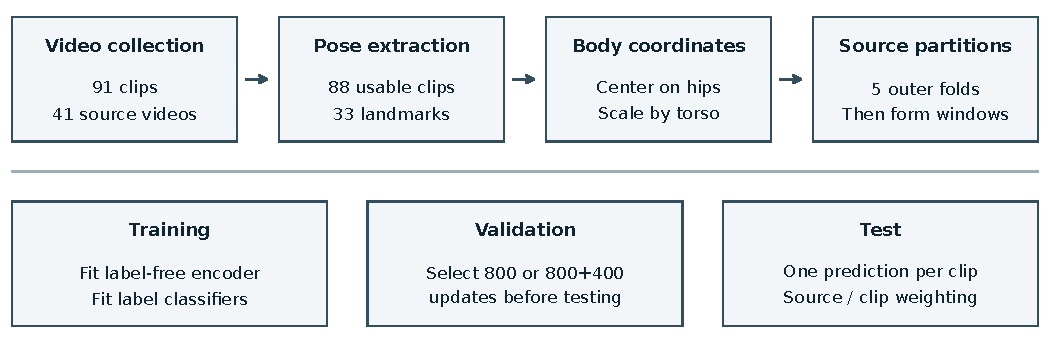
\includegraphics[width=\textwidth]{figures/pipeline-v5.pdf}
\caption{The notebook-defined evaluation. Pose extraction precedes body-relative normalization. Source partitions are fixed before window generation; encoder training and label-classifier fitting use only training sources, and validation chooses the training stage. Test predictions are pooled under two explicitly defined weighting rules.}
\label{fig:pipeline}
\end{figure*}

\section{Video collection and pose processing}
The collection contains 91 downloaded MP4 clips grouped by an 11-character source-video identifier. The labels Normal, MS, and PD describe collection metadata, not diagnoses established by this study. Pose cleaning retains 88 clips from 41 sources (Table~\ref{tab:data}). A source identifier is a recording identifier: different sources may contain the same participant, while one source may contain more than one person. Neither possibility is resolved by the available metadata.

\begin{table}[t]
\centering
\caption{Collection composition. A padded clip has fewer than 32 retained frames. Windows overlap within a clip and are not independent observations.}
\label{tab:data}
\small
\setlength{\tabcolsep}{4pt}
\begin{tabular}{lrrrrr}
\toprule
Label & Raw & Usable & Sources & Padded & Windows\\
\midrule
Normal &26&24&16&5&59\\
MS &30&29&13&0&171\\
PD &35&35&12&10&128\\
\midrule
Total &91&88&41&15&358\\
\bottomrule
\end{tabular}
\end{table}

The extraction pipeline uses MediaPipe pose estimation from the BlazePose family~\cite{blazepose}. It processes full frames and retains the first detected pose. The cached array has 33 landmarks with pixel $x$, pixel $y$, and a visibility value for each sampled frame. Visibility is the detector's estimate of whether a landmark is visible; it is neither a clinical confidence score nor an independently measured quality rating. The pose-estimator interface converts its image-normalized coordinates to pixels before caching; the subsequent body-relative normalization described below is a separate operation. Depth is not used.

Frames are selected with integer stride $\max(1,\operatorname{round}(f_{\rm src}/15))$. Thus, 15 frames per second is a nominal target rather than an exact common sampling rate. Windows contain the same number of sampled frames but can cover different lengths of time. Cleaning requires finite $x$ coordinates for every landmark in at least 30\% of sampled frames, trims empty ends, and interpolates missing coordinates and visibility within the sequence. No maximum interior gap length is imposed. At least eight frames must survive cleaning. Three clips are excluded, but the saved exclusion list does not identify a separate failure criterion for each.

For pixel position $x_{tj}\in\mathbb{R}^2$, hip midpoint $h_t$, and shoulder midpoint $s_t$, the normalized coordinates are
\begin{equation}
\widetilde{x}_{tj}=\frac{x_{tj}-h_t}{\max(\|s_t-h_t\|_2,10^{-3})}.
\label{eq:normalization}
\end{equation}
Spatial normalization leaves the already cleaned visibility values unchanged. This transformation removes absolute pelvis translation and apparent torso size. Within each frame it preserves defined angles under a common positive scale, but frame-varying scale changes displacement over time. The resulting trajectories are not calibrated measurements of physical speed or stride length.

Each source is assigned to a partition before generating 32-frame windows with stride 16. A shorter clip is padded by repeating its final frame. There are 358 windows in total, including 15 padded clips. Padding and interpolation can change apparent dynamics. Table~\ref{tab:data} reports the padding counts by label; the retained caches do not provide per-label counts or gap lengths for interpolation.

\section{Predictive skeleton representation}
\subsection{Stochastic region masking}
A training window contains all 33 landmarks and three channels. Four consecutive frames for one landmark form a token, giving eight time blocks and $8\times33=264$ tokens. A mask marks positions whose observations are withheld from the context network and whose features are predicted; the remaining positions provide context. The sampler operates on seven overlapping regions: head, mouth, left arm, right arm, trunk, left leg, and right leg. It draws one region and a contiguous span of one to six time blocks, adds their tokens to the target set, and repeats until it reaches the rounded target budget of 158 tokens (nominally 60\%) or after 36 region draws. Span length and admissible start position are drawn uniformly. Region overlap and the final draw mean the realized target fraction can exceed 60\%.

Twelve landmarks influence region-selection weights: both shoulders, hips, knees, ankles, heels, and foot indices. A region containing any of these landmarks receives a factor of 1.5, divided by the average number of regions containing its constituent joints; the resulting weights are normalized over regions. This is a bias in region selection. It neither fixes which joints are masked nor makes each highlighted joint 1.5 times as likely to be hidden. Shoulders and hips appear in two regions, so the overlap correction does not equalize their final masking frequencies.

The arms also receive the boost because they contain shoulders, so their elbows, wrists, and hand landmarks inherit that region weight. Every example receives a new mask. The sampler guarantees at least one visible token from the twelve-landmark set somewhere in the window, as well as nonempty target and context sets. The retained token can be a shoulder: neither hip nor leg context is guaranteed even somewhere in a particular window, and an entire time block can be hidden. In the notebook's separate seed-zero bank of 512 masks, the mean target fraction is 63.3\%, and every joint is visible somewhere in at least 74.0\% of windows. These sampler diagnostics describe draws from the rule, not realized exposure in the five-fold training run. The anatomical choice is a design hypothesis motivated by gait analysis. No comparison with uniform, motion-dependent, or alternative anatomical masking establishes its benefit.

\subsection{Learning to predict hidden features}
The encoder converts each group of four frames for one landmark into a 96-number feature vector. Learned position codes specify the landmark and time block. Transformer layers combine information across visible positions, and a second network predicts features at the hidden positions. A reference network, called the target encoder, supplies those training targets. It starts as a copy of the context encoder and is updated gradually toward its weights through an exponential moving average (EMA). This makes the targets change more slowly than the network being optimized. Table~\ref{tab:settings} records the architecture and optimization settings.

\begin{table}[t]
\centering
\caption{Settings for the evaluated model. Both training stages use the same architecture and loss; the continuation restarts optimization state.}
\label{tab:settings}
\small
\setlength{\tabcolsep}{4pt}
\begin{tabular}{p{.43\columnwidth}p{.49\columnwidth}}
\toprule
Setting & Value\\
\midrule
Input window & $32\times33\times3$\\
Frames per landmark token & 4 (12 input values)\\
Encoder / predictor depth & 3 / 2 transformer layers\\
Feature width / attention heads & 96 / 4\\
Feed-forward expansion / dropout & 2 / 0\\
Batch size / training updates & 32 / 800, then 400\\
AdamW peak rate / weight decay & $10^{-3}$ / 0.05\\
AdamW coefficients / norm clip & $(0.9,0.95)$ / 1\\
Learning-rate schedule & 10\% warmup, cosine decay\\
EMA momentum & Cosine, 0.996 toward 1\\
Center momentum & 0.9\\
Prediction / target temperature & 0.10 / 0.06\\
Initialization and training seed & 42\\
\bottomrule
\end{tabular}
\end{table}

The context network receives a geometrically transformed window. Rotation is sampled within $\pm15^\circ$, scale within $[0.9,1.1]$, and translation within $\pm0.1$ body-normalized units per axis. Horizontal reflection occurs with probability 0.5 and exchanges left and right landmark slots, including their visibility values. One transform applies to the whole window. To withhold the hidden observations, visible positions cannot draw information from target positions in the context encoder. The implementation enforces this through an attention mask and replaces hidden-position outputs with a shared learned placeholder before prediction. The predictor also receives joint and time position codes, so different hidden positions can receive different predictions. The target encoder receives the complete, untransformed window and changes only through weight averaging. The loss compares predicted and target distributions over the 96 feature dimensions at masked slots; these distributions are not class probabilities.

Training penalizes disagreement between predicted and reference features. Each 96-number vector is converted to nonnegative weights that sum to one, and cross-entropy measures how closely the two distributions agree. A running mean centers the reference features before this conversion; the temperature settings in Table~\ref{tab:settings} control how concentrated the distributions become. We first average the error over hidden positions within a window, then give each window equal weight in its batch. The running mean is updated once per batch from all masked reference vectors, so this centering step weights token positions equally. The exact equations and update rules appear in the companion methods record, \texttt{evidence/method-details.md}.

Training samples windows with replacement so that each training source has equal total probability. The batch size is 32, with 800 initial updates and a 400-update continuation on the same training sources. Both stages use all training sources and the same prediction task, without condition labels in the encoder loss. Continuation retains network weights but resets the optimizer, center, random streams, and schedules. It therefore differs from uninterrupted training for 1,200 updates.

The settings in Table~\ref{tab:settings} define the evaluated configuration. They do not describe an independently optimized architecture.

\subsection{From learned features to a clip label}
For classification, we keep the target encoder's weights fixed and supply every token of the complete window. We average its features at the 161 token positions selected by one fixed mask drawn with seed zero, then average window vectors within each clip. The mask here selects output positions; it does not hide the corresponding input coordinates. All 33 landmarks occur at least once in the selected positions. The result is one 96-dimensional vector per clip.

Each feature is standardized using training clips only, then a logistic-regression classifier is fitted to their labels ($C=1$, maximum 2,000 iterations, seed 42). This is a linear classifier: it combines the feature values with learned weights. Class weighting gives greater fitting weight to labels with fewer training clips. Each training stage has its own classifier. Validation source-weighted macro-F1 selects the stage, with ties retaining the initial stage; the chosen model is then applied to outer-test clips. The scaler, classifier, and encoder are not refit on combined training and validation sources. These class weights do not equalize recordings within a label: a source with many clips still has more influence on classifier fitting than a source with one clip.

\section{Evaluation}
\subsection{Partitions and baselines}
We sort the source identifiers and divide one row per source into five groups using shuffled, label-stratified splitting (\texttt{StratifiedKFold}). The procedure distributes the three labels across groups, then expands source assignments to clips. Each group serves once as the outer test set, or fold. Among the other sources, the first split from a four-fold version of the same procedure forms a separate validation group for choosing the training stage. The outer seed is 42 and the inner seed is $43+k$ for fold $k$. This gives five test evaluations, each with one validation group; we do not search across every possible inner split. Every retained clip has exactly one outer-test prediction.

\begin{table}[t]
\centering
\caption{Source/clip counts in the fixed partitions.}
\label{tab:splits}
\begin{tabular}{crrr}
\toprule
Fold & Training & Validation & Test\\
\midrule
0&24/51&8/19&9/18\\
1&24/58&9/17&8/13\\
2&24/54&9/17&8/17\\
3&24/53&9/21&8/14\\
4&24/45&9/17&8/26\\
\bottomrule
\end{tabular}
\end{table}

Mean pose averages normalized $x,y$ over each complete clip, yielding 66 features without temporal order. Visibility uses the mean and standard deviation of each landmark's visibility, also yielding 66 features. Both use the same linear-classifier recipe as the learned representation. Mean pose retains posture and viewing geometry, while visibility may reflect occlusion, body orientation, or detector behavior. Neither is a pure measurement of recording conditions.

The engineered-feature baseline reads cleaned pixel coordinates. Its intended vector contains six per-side hip, knee, and ankle angle means, three absolute bilateral mean differences, and six per-side ranges. The legacy container has 82 fields, but only 15 columns vary in each training fold along this extraction route. In the notebook-reported experiment, the left-ankle range duplicates the right-ankle range. This omits one intended measurement and limits conclusions about the intended baseline. A Random Forest (RF) combines the predictions of decision trees fitted to these measurements. Here it uses 100 trees, maximum depth five, square-root feature subsampling, class-balanced training, and seed 42. Columns constant in the training partition are removed, and the remaining features are standardized using that partition. A majority-class baseline predicts the most frequent training-clip label in each fold. All methods use identical outer partitions, but the S-JEPA procedure additionally selects between two stages on validation data. These are comparisons of complete procedures: they do not isolate the effect of temporal information alone.

\subsection{Comparing predictions}
F1 balances how often a predicted label is correct with how many examples of that label are found. We calculate it separately for Normal, MS, and PD, then average the three values to obtain macro-F1. Higher values indicate better classification, with one representing perfect predictions. The score is different from the fraction of correctly classified clips.

Our main comparison gives every source recording equal total weight, preventing a recording with many clips from dominating the result. Each clip from a source with $n_s$ clips receives weight $1/n_s$; for example, the 13 clips from one MS source each receive weight $1/13$. We combine all held-out predictions using these weights before calculating macro-F1. We also give every clip equal weight in a second comparison. The final column of Table~\ref{tab:results} reports the mean score across the five test groups and their standard deviation (SD), which describes how much those scores vary. Averaging the group scores can give a different value from scoring all predictions together.

We additionally check how the results depend on which recordings are included by resampling whole sources and recalculating scores 10,000 times. All clips from a sampled source stay together, each label retains its source count, and all methods use the same sampled sources. The middle 95\% of these recalculated differences is reported once in Results. This check uses saved predictions rather than retraining the models. Exact formulas, seed and resampling details are provided in \texttt{evidence/v9-methods.md}, together with the limits of this additional analysis.

\section{Results}
Table~\ref{tab:results} reports the primary notebook-defined experiment, verified against all 88 saved test predictions. S-JEPA reaches macro-F1 0.457 when recordings receive equal weight, compared with 0.411 for the handcrafted joint-angle RF---an observed improvement of 0.0454. Its features also give higher scores than the tested visibility-only and majority-label baselines. A linear classifier can therefore use the trained representation to predict collection labels on held-out source recordings. This is a useful result for a compact model trained on only 45--58 clips per split.

\begin{table}[t]
\centering
\caption{Held-out macro-F1. Source and clip columns pool all outer-test predictions; the last column summarizes source-weighted fold scores. SD is descriptive. $^*$The notebook RF contains a duplicated ankle-range feature.}
\label{tab:results}
\small
\setlength{\tabcolsep}{4pt}
\begin{tabular}{lrrr}
\toprule
Representation & Source & Clip & Fold mean $\pm$ SD\\
\midrule
S-JEPA &0.457&0.397&$0.438\pm0.196$\\
Mean pose &0.452&0.410&$0.427\pm0.132$\\
Joint angles + RF$^*$ &0.411&0.397&$0.395\pm0.098$\\
Visibility &0.318&0.318&$0.285\pm0.104$\\
Majority class &0.259&0.202&$0.159\pm0.022$\\
\bottomrule
\end{tabular}
\end{table}

Mean pose provides a strong comparison, reaching 0.452 when recordings receive equal weight. The S-JEPA lead over it is 0.0047. When clips receive equal weight, mean pose reaches 0.410, while S-JEPA and the notebook RF both round to 0.397; RF is slightly higher before rounding. Mean pose and RF each correctly classify 37 clips, compared with 36 for S-JEPA. The advantage over RF thus concerns the equal-recording score, rather than the number of correctly classified clips. This distinction matters because one MS recording contributes 13 clips.

\begin{figure*}[t]
\centering
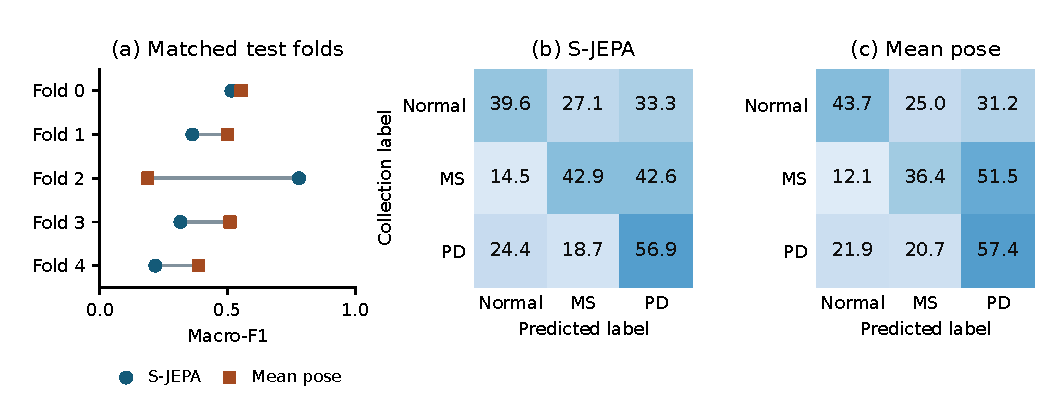
\includegraphics[width=\textwidth]{figures/folds-and-errors-v5.pdf}
\caption{Notebook-associated outer-test results. (a) Source-weighted macro-F1 in each test fold. A straight line joins the two methods evaluated on the same sources; circles denote S-JEPA and squares mean pose. (b,c) Row-normalized source-weighted confusion percentages. Rows are collection labels, columns predictions, and each source contributes total weight one before row normalization. These are not percentages of clinically verified patients.}
\label{fig:results}
\end{figure*}

Performance varies across the test groups (Figure~\ref{fig:results}a). S-JEPA scores range from 0.217 to 0.780, and mean pose is higher in four of the five groups. Mean pose retains average body configuration and can reflect time spent in different positions even though it discards their order, which helps explain why it is an informative control for a sequence model. S-JEPA correctly classifies 10/24 Normal, 8/29 MS, and 18/35 PD clips. When recordings receive equal weight, the corresponding fractions of each label recovered are 0.396, 0.429, and 0.569 (Figure~\ref{fig:results}b). These class-level results identify substantial room to improve all three predictions.

Resampling the saved predictions gives a middle-95\% range of $[-0.133,0.220]$ for the S-JEPA minus RF difference and $[-0.160,0.174]$ for S-JEPA minus mean pose. These ranges show that the observed score advantages can change with the sampled recordings. They describe variation within this collection while holding the trained models fixed; they do not establish how either method will perform in a new clinical population. The complete calculation, including the S-JEPA score range $[0.329,0.579]$, is retained in the companion methods record.

Validation selects the initial training stage in test groups zero through two and the continued stage in groups three and four. The choice follows classification performance on separate validation recordings.

The primary comparison follows the protocol and written results in the top-level notebooks. We verified these results against the matching saved predictions; the notebook's evaluation code has no saved cell outputs. The companion audit record (\texttt{evidence/reproducibility.md}) names the notebook-associated execution and separately identifies the corrected verification. It records input hashes and the command for \texttt{evidence/results\_audit.py}, which recomputes every table metric and interval into \texttt{results-audit.json}.

\subsection{Separate verification of the RF correction}
A later saved evaluation uses the true left-ankle range in place of the duplicated right-ankle range. As a manuscript-stage verification, we refit the small deterministic RF baseline on the existing partitions. Current extraction reproduces all 88 later predictions, and replacing only that feature with the historical duplicate reproduces all 88 notebook-associated RF predictions. Twelve predictions change between versions. This identifies the feature correction as sufficient to reproduce the RF difference under these settings, while preserving both records.

The corrected RF gives macro-F1 0.325 when recordings receive equal weight and 0.321 when clips receive equal weight, compared with 0.411 and 0.397 for the notebook-reported version. S-JEPA remains higher under equal-recording scoring, with a difference of 0.1314; its resampling range is $[-0.046,0.304]$. The feature correction lowers this RF score, illustrating why feature correctness must be checked independently of the resulting accuracy. Both executions use the same data, split, and training seed, and their S-JEPA predicted labels coincide despite different feature vectors. This is a verification of the baseline implementation, rather than an independent repetition with new seeds or recordings. It compares the specific RF settings used here and does not cover more extensively tuned classical gait systems.

\section{Discussion and limitations}
The study supports the practical use of trained skeleton features for predicting labels in a small gait-video collection. The encoder receives no condition labels during feature training, yet its fixed numerical descriptions can be used by a linear classifier on held-out recordings. Under equal-recording scoring, this combination exceeds the tested handcrafted joint-angle RF, including its separately verified feature correction. The result offers a concrete reason to investigate predictive skeleton features alongside established gait summaries when recordings are limited.

The observed benefit applies to these complete procedures. S-JEPA and the RF differ in feature construction and classifier, and only S-JEPA selects between two training stages. Their score difference therefore cannot identify which component accounts for the gain. Here, useful features means information that supports prediction of the supplied collection labels; their relationship to specific movement impairments remains to be established. Comparing the trained encoder with the same network at initialization would measure what training adds. Testing a matched change in frame order would help determine the contribution of movement sequence. Neither experiment was performed here. Mean pose's competitive results make it a valuable reference in those follow-up comparisons.

A known implementation issue concerns reflection during training. Reflection exchanges left and right landmark slots in the context input, while the mask and unreflected target retain their original indices. A physical joint selected as a target can consequently remain visible in the opposite-side context slot. This mismatch occurs within training examples; its effect on classification was not measured. A comparison with corrected correspondence or with reflection disabled would determine its importance. The anatomical mask choice likewise remains a design hypothesis without a separate performance comparison.

The collection is small and heterogeneous, and the training uses one random seed. Different source identifiers may still contain the same participant, and the supplied labels are not verified diagnoses. Viewpoint, pose-estimation errors, interpolation and repeated-frame padding can all influence the input. Body normalization removes absolute pelvis movement and apparent torso size, so the learned descriptions are not calibrated measurements of walking speed or stride length. The visibility-only comparison cannot rule out recording-related information in the other representations.

The available records do not establish participant consent for secondary health inference, a complete assessment of source-media rights, or an ethics-review determination. These require documentation before a release or clinical follow-up. The present predictions do not support individual clinical decisions. A larger study with verified identities and diagnoses could assess transfer to new participants and recording sites, and test whether predicted confidence agrees with observed accuracy.

\section{Conclusion}
A compact S-JEPA pipeline trained on a small collection of gait videos produced features that supported prediction of the collection labels on held-out source recordings. It achieved the highest observed macro-F1 when each recording received equal weight: 0.457, compared with 0.411 for the tested handcrafted joint-angle RF and 0.452 for mean pose. This modest observed improvement over the RF provides an encouraging starting point for predictive skeleton learning with limited video data. The strong mean-pose comparison and documented implementation checks provide a clear basis for the next experiments: establish what training and frame order add, then assess the resulting features in an independent, clinically verified collection.

{\small
\bibliographystyle{ieeenat_fullname}
\bibliography{references-v9}
}
\end{document}
